%\documentclass[aspectratio=169]{beamer}
\documentclass{beamer}
% \usepackage{beamerthemesplit} // Activate for custom appearance
\usetheme {Dresden}
\usepackage[utf8]{inputenc}
\usepackage{etoolbox}


\usenavigationsymbolstemplate{}

\addtobeamertemplate{footline}{centered}
{%
   \usebeamercolor[fg]{author in sidebar}
   \vskip-1cm
\hspace*{\fill} Spezifikationsvortrag Softwareprojekt - Graphbasierte Methode zur Generierung von deutschen Lexika für Hate Speech \hspace*{\fill}%
\llap
   \insertframenumber\,/\,\inserttotalframenumber\kern1em\vskip2pt%
}

\begin{document}

\title[]{Spezifikationsvortrag}
\author[]{Fabian Düker, Uli Steinbach}
\institute{Universität Heidelberg, Institut für Computerlinguistik\linebreak\vspace{0.03\textwidth}
Softwareprojekt, SoSe 2018\linebreak\vspace{0.02\textwidth}
Prof Dr. Katja Markert}
\date{12.06.2018}

\frame{\titlepage}
\begin{frame}[allowframebreaks]{Übersicht}
\tableofcontents
\end{frame}


%%%%%%%%%%%%%%%%%%%% SECTION 1 %%%%%%%%%%%%%%%%%%%%%%%%%%%%%%%%%%%%%%%%%%%%%%%%%%%%%%%%%%%%%%%%%%%%%%%%%%%%%%%

\section{Übersicht}

\subsection[Aufgabe]{Aufgabe }

\begin{frame}{Übersicht}
\begin{block}{Autom. Erstellung eines Lexikons für die Erkennung von Abusive Words }
Anwendung auf Germeval 2018 Task I $\Rightarrow$ Binäre Klassifikation von 5000 Tweets 
\end{block}
\end{frame}


\section{Inhaltliche Spezifikation}
\subsection[inh. Spez.]{ inh. Spezifikation }

\begin{frame}{Problemstellung}
\begin{itemize}
	\item Problem: Hatespeech ist in ständiger Veränderung begriffen (Neologismen, Ambiguität, Kontext/Domäne)
	\item Wiegand et al. 2016: Erstellung eines englischen Lexikons mit guten Ergebnissen auf cross-domain Evaluation
	\item Erstellung eines kontextunabhängigen Lexikons für das Deutsche
	\item Anwendung des Lexikons bei der (binären) Erkennung von Tweets
%	\item SentiWS: Lexikon mit negativen Wörtern für das Deutsche

\end{itemize}
\end{frame}

\begin{frame}{Lösungsansatz}
\begin{itemize}
\item manuelle Erstellung Baselexikon aus SentiWS neg. Sentiment-Lexikon
\item Halbautomatische Erweiterung des Baselexikons mit deutschen Schimpwörtern
\item Autom. Erweiterung mittels graphbasiertem Label-Propagation-Algorithmus
\item Anwendung auf Germeval 2018 Datenset und Evaluation
\end{itemize}
\end{frame}
\begin{frame}{Erstellung des Baselexikons}
\begin{block}{SentiWS}
	\begin{itemize}
		\item Extraktion negativer Wörter aus SentiWS
		\item 686 Nomen
		\item 420 Verben
		\item 708 Adjektive
		\item Problem: Zu wenige explizite Schimpfwörter
		\item Lösung: Mehr Schimpfwörter hinzufügen
	\end{itemize}
\end{block}
\end{frame}

\begin{frame}{Erstellung des Baselexikons}
\begin{itemize}
\item Genius API: Erstellung eines Deutschrapkorpus 
\item Deutschrap: zeitgemäße Verwendung von Schimpfwörtern (genrespezifisch, aber auch politisch, rassistisch, sexistisch)
\item autom. Extraktion von Kandidaten mittels syntaktischer Pattern
\end{itemize}
\end{frame}

\begin{frame}{Erstellung des Baselexikons}
	\begin{itemize}
		\item Automatischer Abgleich aller Nomen im Rapkorpus
		\item mit Schimpfwortliste aus dem Internet
		\item mit Pattern "du [NN]"
		\item etwa 280 potentielle Schimpfwörter
		\item manuelles Aussortieren von false positives (z.B. "Rapper")
		\item Auswahl der 200 häufigsten Schimpfwörter
		\item Erweiterung durch beleidigende Adjektive
		\item Suche nach Pattern "du [ADJ] Schimpfwort"
		\item etwa 280 potentiell beleidigende Adjektive
	\end{itemize}
\end{frame}

\begin{frame}{Erstellung des Baselexikons}
	\begin{itemize}

		\item Lemmatisierung mit IWNLP
		\item Lemmatisierung der nicht erkannten Adjektive von Hand
		\item Beseitigung von Duplikaten
		\item Finales Baselexikon:
		\item 887 Nomen
		\item 413 Verben
		\item 824 Adjektive
		\item  - 2124 Wörter

	\end{itemize}
\end{frame}

\begin{frame}{Rapkorpus}
\begin{itemize}
\item Texte von 30 Rappern (Auswahl angelehnt an Daten-Journalismus Studie des BR/PULS zum Thema "Diskriminierung im Deutschrap" aus dem Jahr 2016)
	\item Bushido
	\item Chakuza
	\item K.I.Z.
	\item Kay One
	\item Kollegah \& Farid Bang
	\item Prinz Pi
	\item Bass Sultan Hengzt
	\item Fler
	\item Azad
	\item Kool Savas
	\item ...

\end{itemize}
\end{frame}

\begin{frame}{Rapkorpus}
Auszug der extrahierten Schimpfwörter vor Handselektion
\begin{itemize}
		
\item \emph{Rapper}
\item \emph{Kopf}
\item \textbf{Arsch}
\item \textbf{Bitch}
\item \textbf{Schwanz}
\item \textbf{Scheiße}
\item \emph{Gangster}
\item \emph{Block}
\item \emph{Baby}
\item \textbf{Nutte}
		
\end{itemize}
\end{frame}


\begin{frame}{Graph-basierter Ansatz für autom. Erweiterung des Baselexikons}
\begin{itemize}
\item Erstellung von pos + neg seed-Liste mit annotierten Schimpwörtern aus Baselexikon (+) und häufigsten Wörtern (-)
\item Graph mit Kanten zw. Wörtern auf Basis von Kosinusähnlichkeit zwischen Word Embeddings Vektoren (auf Twitter Korpus trainiert)
\item Propagierung der Seed-Labels auf ungelabelte Knoten/Wörter mittels graphbasiertem Label-Propagation-Algorithmus (Adsorption Algorithmus, Talukdar et al. 2008)
\end{itemize}
\end{frame}

\begin{frame}[plain, t]
{Graph-basierter Ansatz für autom. Erweiterung des Baselexikons}
\bigskip
\bigskip
\center
\begin{figure}[hbt]
    \begin{center}
        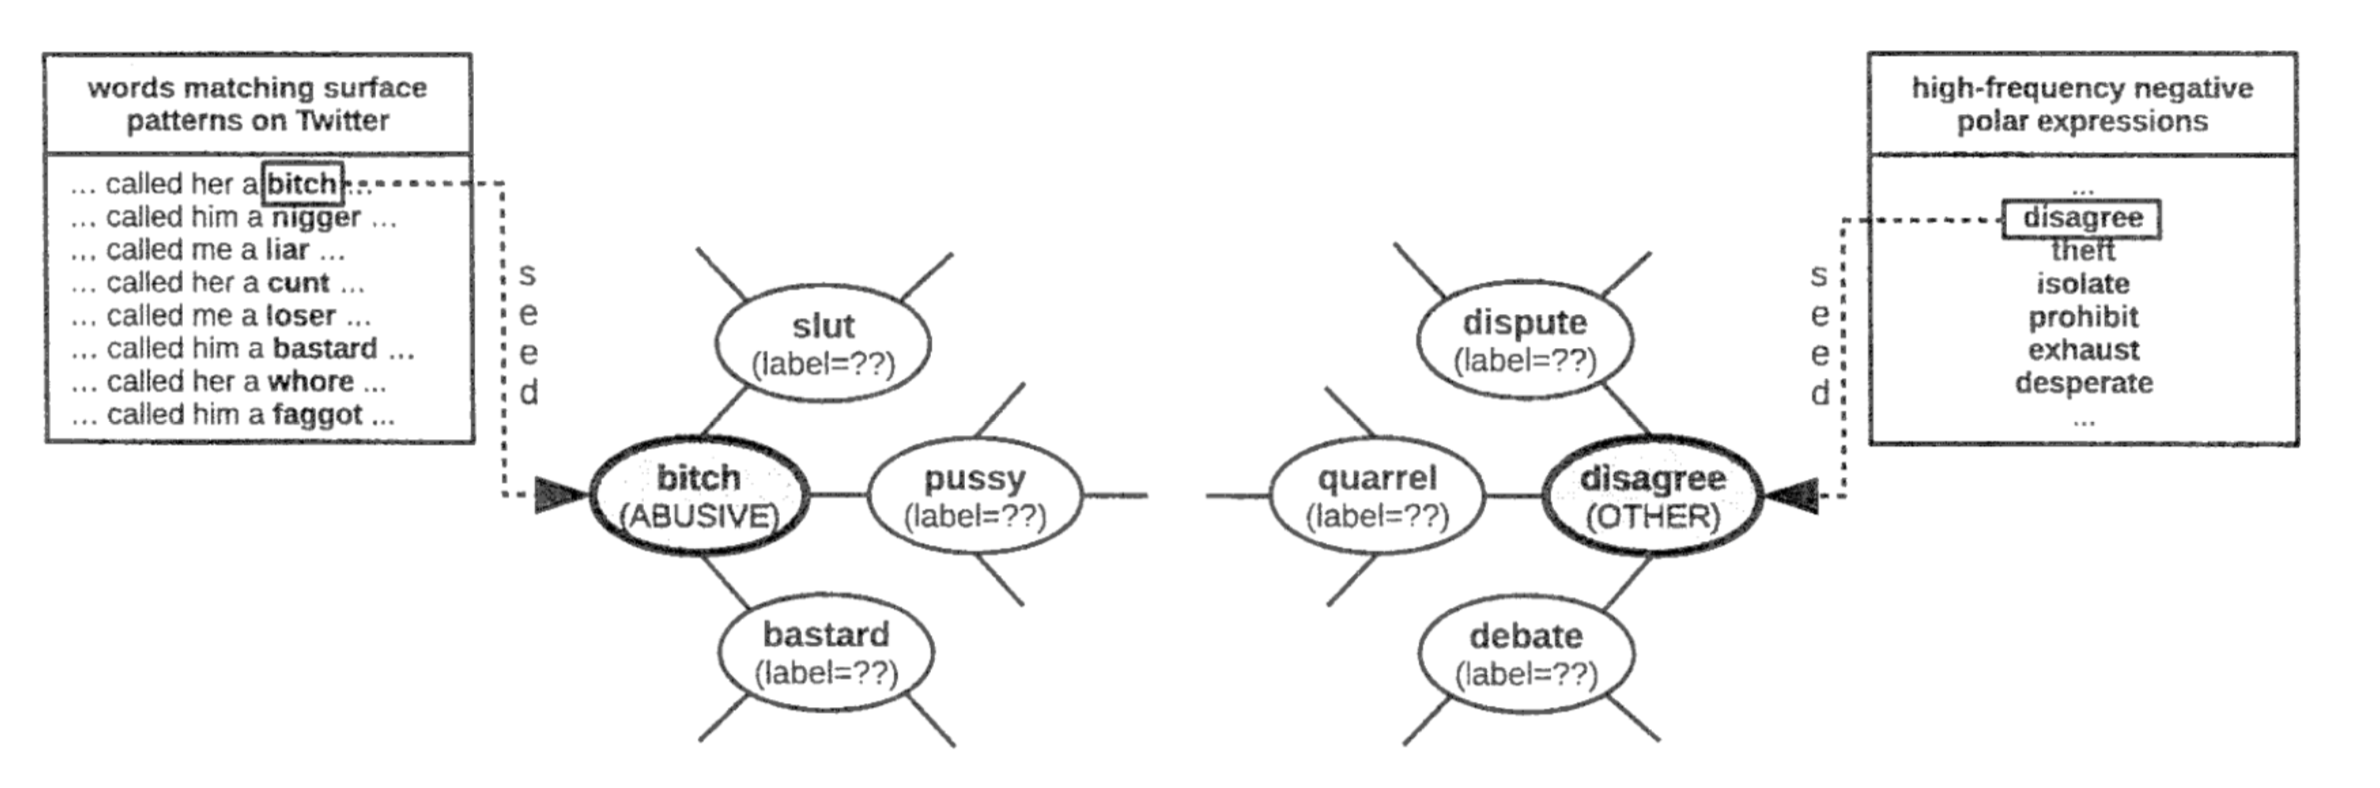
\includegraphics[width=\textwidth,height=0.95\textheight,keepaspectratio]{graph.png}\\
    \end{center}
\caption{Label Propagation Graph aus Wiegand et al. 2018}\label{preprocess}
\end{figure}

\end{frame}

%%%%%%%%%%%%%%%%%%%%%%%%%%%%%%%%%%%%%%%% EVALUATION %%%%%%%%%%%%%%%%%%%%%%%%%%%%%%%%%%%%%%%%%%%%%%%%%%%%%%%%%%%%%%%%%%%%%%%%%


\begin{frame}[fragile]{Anwendung und Evaluation auf Germeval Datenset}
\begin{itemize}
\item Germeval 2018: deutschsprachiger Twitter Korpus $\Rightarrow$ 5000 annotierte Tweets bzgl. beleidigender Sprache
\item Task I: binäre Klassifikation der Tweets
\item \textbf{beleidigend:} \\ \footnotesize \texttt{Für mich ist die \#katholische \#Kirche nur ein Sammelbecken von \#Verbrechern \#Kinderschändern und \#Kriminellen}
\item \normalsize \textbf{other:} \\ \footnotesize \texttt{Endlich hat Kurz einen Verbündeten aus Frankreich, der auch die LBR ungesetzliche Einwanderung von jungen Afrikanern unterbinden will}
\end{itemize}
\end{frame}

\begin{frame}[fragile]{Anwendung und Evaluation auf Germeval Datenset}
\begin{itemize}
\item Unser Ansatz für die Verwendung des Baselexikons und warum könnte das besser sein ?
\end{itemize}
\end{frame}

\begin{frame}{Baseline}
\begin{itemize}
\item Baseline 1: Majority Baseline
\item Baseline 2: Unigram und Bigram SVM
\item Baseline 3: Feature Selection (Mutual Information) SVM 
\item Preprocessing: Autosarkasmus-SP (SoSe 2016): Alle Tweets wurden tokenisiert, normalisiert und pos-getagged. Zusätzlich Lemmatisierung und stopword removal
\item 10-Fold Cross Validation mit random-seed für bessere Vergleichbarkeit
\end{itemize}
\end{frame}

\begin{frame}{Baseline}
\begin{itemize}
\item Unigram und Bigram SVM: Input-Features sind die auf der Dokument-Term Matrix berechneten tf-idf Werte für Uni- bzw. Bigramme.    
\item Feature Selection Algorithmus: Berechnung des mutual information score (Manning et. al 2011) zwischen Label und Wort $\Rightarrow$ 1500 Wörter mit den höchsten mi-scores als Input-Features für SVM Klassifizierer. 
\end{itemize}
\end{frame}


%%%%%%%%%%%%%%%%%%%%%%%%%%%%%%%%%%%%%%%%%%%% TABLE 1 %%%%%%%%%%%%%%%%%%%%%%%%%%%%%%%%%%%%%%%%%%%%%%%%%%
\begin{frame}[plain,t]{Evaluation der Baseline}
\begin{table}[]
\centering
\caption{Baseline: tf-idf unigram SVM}
\label{my-label}
\resizebox{\textwidth}{!}{%
\begin{tabular}{|l|l|l|l|l|l|l|l|l|l|}
\hline
Fold & \#train & pos & neg & tok/tw & \#test & pos & neg & tok/tw & F1 \\ \hline
1 & 4500 & 1524 & 2976 & 146.94 & 500 & 160 & 340 & 144.124 & 0.7026952348344236 \\ \hline
2 & 4500 & 1560 & 2940 & 146.73 & 500 & 124 & 376 & 146.05 & 0.7430423747345847 \\ \hline
3 & 4500 & 1525 & 2975 & 146.73 & 500 & 159 & 341 & 146.0 & 0.6822048536263124 \\ \hline
4 & 4500 & 1505 & 2995 & 146.57 & 500 & 179 & 321 & 147.512 & 0.6637390819218496 \\ \hline
5 & 4500 & 1498 & 3002 & 145.94 & 500 & 186 & 314 & 153.154 & 0.6466493970138341 \\ \hline
6 & 4500 & 1504 & 2996 & 147.0 & 500 & 180 & 320 & 143.568 & 0.6675527979162865 \\ \hline
7 & 4500 & 1504 & 2996 & 146.61 & 500 & 180 & 320 & 147.106 & 0.6563892890626787 \\ \hline
8 & 4500 & 1519 & 2981 & 146.16 & 500 & 165 & 335 & 151.13 & 0.6681861534976389 \\ \hline
9 & 4500 & 1504 & 2996 & 147.08 & 500 & 180 & 320 & 142.86 & 0.650127611518916 \\ \hline
10 & 4500 & 1513 & 2987 & 146.83 & 500 & 171 & 329 & 145.104 & 0.6737827241885149 \\ \hline
\multicolumn{10}{|r|}{\bf{Total Accuracy: 0.68 (+/- 0.05)}} \\ 
\hline
\end{tabular}%
}
\end{table}

\end{frame}
%%%%%%%%%%%%%%%%%%%%%%%%%%%%%%%%%%%%%%%%%%%% TABLE 2 %%%%%%%%%%%%%%%%%%%%%%%%%%%%%%%%%%%%%%%%%%%%%%%%%%
\begin{frame}[plain, t]{Evaluation der Baseline}
\begin{table}[]
\centering
\caption{Baseline: tf-idf bigram SVM}
\label{my-label}
\resizebox{\textwidth}{!}{%
\begin{tabular}{|l|l|l|l|l|l|l|l|l|l|}
\hline
Fold & \#train & pos & neg & tok/tw & \#test & pos & neg & tok/tw & F1 \\ \hline
1 & 4500 & 1524 & 2976 & 146.94 & 500 & 160 & 340 & 144.124 & 0.6713317445366677 \\ \hline
2 & 4500 & 1560 & 2940 & 146.73 & 500 & 124 & 376 & 146.05 & 0.7143231005141465 \\ \hline
3 & 4500 & 1525 & 2975 & 146.73 & 500 & 159 & 341 & 146.0 & 0.6607936275023581 \\ \hline
4 & 4500 & 1505 & 2995 & 146.57 & 500 & 179 & 321 & 147.512 & 0.6407256780069586 \\ \hline
5 & 4500 & 1498 & 3002 & 145.94 & 500 & 186 & 314 & 153.154 & 0.6004567364407795 \\ \hline
6 & 4500 & 1504 & 2996 & 147.0 & 500 & 180 & 320 & 143.568 & 0.636733440679629 \\ \hline
7 & 4500 & 1504 & 2996 & 146.61 & 500 & 180 & 320 & 147.106 & 0.6211176439430055 \\ \hline
8 & 4500 & 1519 & 2981 & 146.16 & 500 & 165 & 335 & 151.13 & 0.6254687762688433 \\ \hline
9 & 4500 & 1504 & 2996 & 147.08 & 500 & 180 & 320 & 142.86 & 0.6184350158030838 \\ \hline
10 & 4500 & 1513 & 2987 & 146.83 & 500 & 171 & 329 & 145.104 & 0.6386443278943279 \\ \hline
\multicolumn{10}{|r|}{\bf{Total Accuracy: 0.64 (+/- 0.06)}} \\ 
\hline
\end{tabular}%
}
\end{table}
\end{frame}

%%%%%%%%%%%%%%%%%%%%%%%%%%%%%%%%%%%%%%%%%%%% TABLE 3 %%%%%%%%%%%%%%%%%%%%%%%%%%%%%%%%%%%%%%%%%%%%%%%%%%


\begin{frame}[plain, t]{Evaluation der Baseline}
\begin{table}[]
\centering
\caption{Baseline: Feature-Selection m. Mutual Information}
\label{my-label}
\resizebox{\textwidth}{!}{%
\begin{tabular}{|l|l|l|l|l|l|l|l|l|l|}
\hline
Fold & \#train & pos & neg & tok/tw & \#test & pos & neg & tok/tw & F1 \\ \hline
1 & 4500 & 1524 & 2976 & 146.94 & 500 & 160 & 340 & 144.124 & 0.7506333288282201 \\ \hline
2 & 4500 & 1560 & 2940 & 146.73 & 500 & 124 & 376 & 146.05 & 0.8159589743589742 \\ \hline
3 & 4500 & 1525 & 2975 & 146.73 & 500 & 159 & 341 & 146.0 & 0.7661802897341697 \\ \hline
4 & 4500 & 1505 & 2995 & 146.57 & 500 & 179 & 321 & 147.512 & 0.761125609472951 \\ \hline
5 & 4500 & 1498 & 3002 & 145.94 & 500 & 186 & 314 & 153.154 & 0.717136006424597 \\ \hline
6 & 4500 & 1504 & 2996 & 147.0 & 500 & 180 & 320 & 143.568 & 0.7715594209711858 \\ \hline
7 & 4500 & 1504 & 2996 & 146.61 & 500 & 180 & 320 & 147.106 & 0.7808015386464718 \\ \hline
8 & 4500 & 1519 & 2981 & 146.16 & 500 & 165 & 335 & 151.13 & 0.7812137931034483 \\ \hline
9 & 4500 & 1504 & 2996 & 147.08 & 500 & 180 & 320 & 142.86 & 0.7738412698412699 \\ \hline
10 & 4500 & 1513 & 2987 & 146.83 & 500 & 171 & 329 & 145.104 & 0.7651150793650793 \\ \hline
\multicolumn{10}{|r|}{\bf{Total Accuracy: 0.77 (+/- 0.05)}} \\
\hline
\end{tabular}%
}
\end{table}
\end{frame}



%%%%%%%%%%%%%%%%%%%%%%%%%%%%%%%%%%%%%%% MODULARISIERUNG %%%%%%%%%%%%%%%%%%%%%%%%%%%%%%%%%%%%%%%%%%%%%%%%%%%%%%%%%%%%%%%%%
\section{Modularisierung und Aufgabenverteilung}
\subsection[Modularisierung]{ Modularisierung und Aufgabenverteilung }

\begin{frame} 
\begin{itemize}
\item Paketierung: Aufsplittung des Gesamtpakets in kleinere Module
\item Python-Pogrammierung (objektorientierte Implementierung)
\item "split und shared tasks"
\end{itemize}
\end {frame}

\begin{frame}[plain, t]
\begin{table}[]
\centering
\label{my-label}
\resizebox{\textwidth}{!}{%
\begin{tabular}{llll}
Modul &  & Uli & Fabian \\
\bf{Erstellung Baselexikon} &  &  &  \\
& Extraktion negativer Wörter aus SentiWS &  & x \\
& Erstellung Rapkorpus & x &  \\
 & PAT-basierte Extraktion von NNs/ADJs & x & x  \\
 & Autom. Abgleich von Nomen mit Schimpfwortliste und Patterns &  & x \\
 & Handselektion der beleidigenden Nomen &  & x \\
 & Lemmatisierung des Lexikons mit IWNLP Lemmatizer &  & x \\
 & Korrektur und Restlemmatisierung des Lexikons &  & x \\
 & Skript für Erstellung eines Annotations-Testsets & x &  \\
  & Skript für autom. Auswertung d. Annotations-Testsets &  & x \\
\bf{Erstellung Baselines} &  &  &  \\
 & Implementation manuelle 10-Fold Cross Validation & x &  \\
 & Integration Autosarkasmus-Tweet Preprocessing & x &  \\
 & Erweitertes Preprocessing (Lemmatisierung, Stopwörter) & x &  \\
 & Implementation Unigram/Bigram SVM Baseline & x &  \\
 & Implementation Mutual Information (Manning et. al 2011) & x &  \\
 & Implementation Feature Selection (MI) SVM Baseline & x &  \\
 & Evaluation und Output & x &  \\
 \bf{Erstellung Word-Similarity Graph} &  &  &  \\
 & Word Embeddings auf Twitter Daten & x & x \\
 & Erstellung des Wortähnlichkeitsgraphen auf Basis von Kosinusähnlichkeiten & x & x \\
 & Unknown Words Handhabung (character-level embeddings?) & x & x \\
 & Erstellung der Seed Listen (pos + neg) & x & x \\
\bf{Label Propagation} &  &  &  \\
 & Implementation Adsorption Algorithmus (Talukdar 2008) & x & x \\
 & Erweiterung des Baselexikons mit Output & x & x \\
\bf{Anwendung und Evaluation} &  &  &  \\
 & Test auf Germeval Daten & x & x \\
 & Verbesserungen und Erweiterungen & x & x \\
 & Visualisierung des Outputs & x & x \\
 & Präsentation der Ergebnisse & x & x \\
 & Abschlussbericht & x & x
\end{tabular}%
}
\end{table}
\end{frame}

%\begin{frame}{Aufgabenverteilung}
%\end{frame}
%
%\begin{frame}{Zeitplan}
%\end{frame}
%
%\section{Programmarchitektur, Datenstrukturen}
%\subsection[Programmarchitektur]{ Programmarchitektur und Datenstrukturen }
%
%\begin{frame}{Programmarchitektur}
%\end{frame}
%
%\begin{frame}{Datenstrukturen}
%\end{frame}



%%%%%%%%%%%%%%%%%%%% SECTION %%%%%%%%%%%%%%%%%%%%%%%%%%%%%%%%%%%%%%%%%%%%%%%%%%%%%%%%%%%%%%%%%%%%%%%%%%%%%%%

\section{Literatur und Ressourcen}
\subsection[Lit. + Res.]{Literatur und Ressourcen}


\begin{frame}{Literatur}
\begin{itemize}
\item Talukdar, Pereira 2008 - Expermiments in Graph-based Semi-Supervised Learning Methods for Class-Instance Acquisition
\item Velikovich et al. 2010 - The Viability of Web-derived Polarity Lexicons
\item Wiegand et al. 2018 - Inducing a Lexicon of Abusive Words - A Feature-Based Approach
\item Manning et al. 2008 - Introduction to Information Retrieval
\item Autosarkasmus SWP 2016 - https://gitlab.cl.uni-heidelberg.de/hoff/GermanTwitterPreprocessing
\item BR/PULS Studie 2016 - https://www.br.de/puls/musik/so-homophob-frauenfeindlich-rassistisch-und-behindertenfeindlich-ist-deutschrap-100.html
\end{itemize}
\end{frame}

\begin{frame}{Ressourcen}
\begin{itemize}
\item \textbf{Schimpfwortliste} http://www.hyperhero.com/de/insults.htm
\item \textbf{SentiWS} http://wortschatz.uni-leipzig.de/en/download/
\item \textbf{Genius API} https://genius.com/
\item \textbf{spaCy} https://spacy.io/
\end{itemize}
\end{frame}



\end{document}
